\documentclass[10pt,aspectratio=169]{beamer}
\usepackage{WHU_Beamer}
%=============导言区==================================================================
\title{presentation}
\subtitle{A Subtitle}
\author{\href{link}{your name}
\\ 
School of Physics, WHU
}
\date{\today}
%=====================================================================================
\begin{document}

\maketitle

\section{Introduction}

\begin{frame}{Acknowledgement}
    \begin{itemize}
        \item 本模板为非官方模板,根据中国科学院大学\href{https://cn.overleaf.com/project/67d429aed396086bd4f730ff}{Jonathan Lin}\cite{url}制作模板修改。校徽校训等来自武大官网。修改了目录页背景的一些bug,增加了中文支持,添加了\texttt{physics}等宏包和例子;
        \item \textcolor{whugreen}{ 请勿用于商业用途!!}
    \end{itemize}
    \begin{figure}[h]
        \centering
        \subfloat[img 1]{
\includegraphics[width=0.3\textwidth]{source/logo.png}}
        \hfill
        \subfloat[img 2]{
\includegraphics[width=0.3\textwidth]{source/logo_blue.png}}
        \hfill
        \subfloat[img 3]{
\includegraphics[width=0.3\textwidth]{source/logo_black.png}}
        \hfill
        \newline
        \caption{图片示例}
    \end{figure}
\end{frame}

\begin{frame}{公式和表格}
    \begin{columns}
        \begin{column}{0.45\textwidth}
        \[ \hat{H} = \left[
        \begin{array}{cccccc}
        v_{11} & -\delta^2  & \cdots &-\delta^2  &\cdots & 0\\
        -\delta^2  & v_{12} & \cdots& \cdots & \cdots & 0\\
        \vdots & \vdots & \vdots & \vdots& \vdots& \vdots \\
        -\delta^2 &0& \cdots &\cdots & \cdots& 0\\
        \vdots &\vdots &\vdots & \vdots &  \vdots & \vdots \\
        0 & 0 & \cdots & \cdots & -\delta^2  &v_{LK}\\
        \end{array} \right] \]
        \end{column}
        \begin{column}{0.55\textwidth}
            \begin{equation}
                \begin{aligned}
                    g(k)&=\frac{1}{\sqrt{2\pi}}\int \Psi(x,0)e^{-ikx}\dd{dx}\\
                    &=\frac{A}{\sqrt{2\pi}}\int e^{-\frac{x^2}{4\sigma^2}e^{-i(k-k_0)x}\dd{x}}\\
                    &=\frac{A}{\sqrt{2\pi}}\int e^{-\frac{1}{(2\sigma)^2}(x+2i(k-k_0)\sigma^2)^2-(k-k_0)^2\sigma^2}\dd{x}
                \end{aligned}
                \label{eq_b}
            \end{equation}
        \end{column}
    \end{columns}
    公式\ref{eq_b}是一个多行公式的例子。
\end{frame}
\begin{frame}[fragile]{表格的例子}
    \begin{minipage}{0.6\textwidth}
    \begin{table}
    \begin{tabular}{c|c}
        \toprule
        \multicolumn{2}{c}{原子单位制} \\[2pt]
        \hline
        质量&$m_e=9.1094\times 10^{-31}kg$\\
        电荷&$e=1.6022\times 10^{-19}C$\\
        角动量&$\hbar=1.0546\times 10^{-43}J\cdot s$\\
        介电常数&$4\pi\varepsilon_0=1.1127\times 10^{-10}F\cdot m^{-1}$\\
        长度&$a_0=\frac{4\pi\varepsilon_0\hbar^2}{m_ee^2}=5.2918\times 10^{-11}m$\\
        能量&$Hartree=\frac{m_ee^2}{(4\pi\varepsilon_0)^2\hbar}=4.3597\times 10^{-18}J$\\
        \bottomrule
    \end{tabular}
\end{table}
\end{minipage}
\begin{minipage}{0.36\textwidth}
    \begin{figure}
        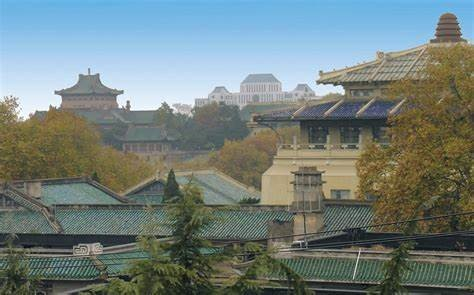
\includegraphics[width=\textwidth]{source/oldphoto.jpg}
        \caption{武大旧景}
    \end{figure}
\end{minipage}
\newline
verb不能出现在\verb|\macro|中,例如\verb|\section|.需要[fragile],或者\verb|\cprotect|
\end{frame}
\section{讨论}
\begin{frame}{非正交基组}
    \begin{itemize}
        \item 通过交叠矩阵的逆矩阵定义非正交基组$|\phi_i\rangle$的对偶基组$|\phi^k\rangle$:
    \begin{equation}
        |\phi^k\rangle=\sum_{i}S^{-1}_{ik}|\phi_i\rangle
    \end{equation}
    \item 运算规则:
    \begin{equation}
        \begin{gathered}
            \langle\phi_j|\phi_k\rangle=S_{jk}\\
            \langle\phi_j|\phi^k\rangle=\delta_{jk}\\
            \langle\phi^j|\phi^k\rangle=S^{-1}_{jk}\\
            \hat{\mathbf{I}}=\sum_{k}|\phi^k\rangle\langle\phi_k|=\sum_{k}|\phi_k\rangle\langle\phi^k|
        \end{gathered}
    \end{equation}
\end{itemize}
\end{frame}
\begin{frame}{切比雪夫多项式}
\subsection{切比雪夫多项式}
为了演化波函数,需要对时间演化算子进行数值展开,由于哈密顿量是稀疏的,所以可以方便地使用Chebyshev多项式进行展开,这种方法对求解含时薛定谔方程是无条件稳定的。假设$x\in[-1,1]$,
\begin{equation}
    e^{-izx}=J_0(z)+2\sum_{m=1}^{\infty}(-i)^mJ_m(z)T_m(x)
\end{equation}
 其中$J_m$是m阶贝塞尔函数,$T_m$是第一类切比雪夫多项式。$T_m(x)$可以由递归关系求解:
\begin{equation}
    T_{m+1}(x)=2xT_{m}-T_{m-1}
\end{equation}
为了利用切比雪夫多项式方法,我们需要将$\hat{H}$缩放为$\tilde{H}=\hat{H}\Vert H\Vert$,使$\tilde{H}$的特征值分布在$[-1,1]$。
\begin{equation}
    |\varphi(t)\rangle=\{J_0(\tau)+2\sum_{m=1}^{\infty}(-i)^mJ_m(\tau)\hat{T}_m(\tilde{H})\}|\varphi(0)\rangle
\end{equation}
$\tau=t\cdot\Vert H\Vert$。
\end{frame}
\begin{frame}[fragile]{代码的例子}
    \begin{lstlisting}[style=C++]
    #include<H5Cpp>
    H5::H5File file(filename, H5F_ACC_RDONLY, H5::FileCreatPropList::DEFAULT, fapl);
    H5::Group group = file.openGroup(group_name);
    H5::DataSet dataset = group.openDataSet(dataset_name);
    H5::DataSpace filespace = dataset.getSpace();
    \end{lstlisting}
    \begin{lstlisting}[style=C++]
    #include<hdf5>
    hid_t plist_id = H5Pcreate(H5P_FILE_ACCESS);
    H5Pset_fapl_mpio(plist_id, MPI_COMM_WORLD, MPI_INFO_NULL);
    hid_t file_id = H5Fopen(filename.c_str(), H5F_ACC_RDONLY, plist_id);
    H5Pclose(plist_id);
    hid_t group_id = H5Gopen(file_id, groupname.c_str(), H5P_DEFAULT);
    hid_t dataset_id = H5Dopen(group_id, dataset_name.str().c_str(), H5P_DEFAULT);                    
    \end{lstlisting}
\end{frame}
\begin{frame}[fragile]{Splitting in Columns}
简单的分栏的例子,注意\verb|textwidth|的变化:\\
\vspace{30pt}
\begin{columns}
    \begin{column}{0.5\textwidth}
        \begin{figure}
            
\includegraphics[width=0.8\textwidth]{source/xiaoxun.png}
        \end{figure}
    \end{column}
    \begin{column}{0.5\textwidth}
        \begin{figure}
            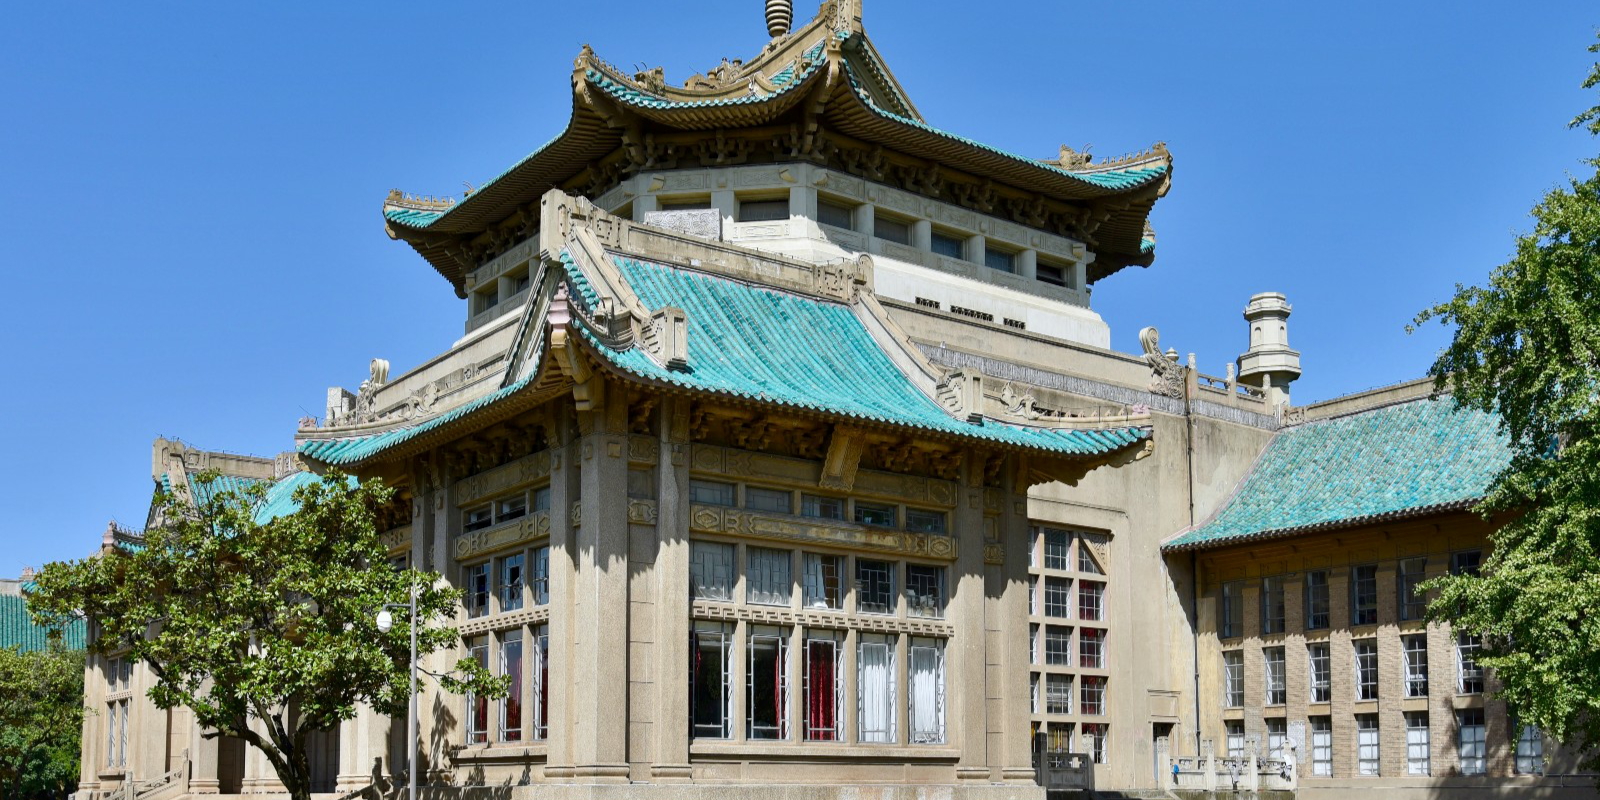
\includegraphics[width=0.8\textwidth]{source/back4.png}
        \end{figure}
    \end{column}
\end{columns}
\end{frame}
\section{Summary}
\begingroup
    \setbeamertemplate{headline}{}
    \setbeamertemplate{footline}{}
    \begin{frame}[c]{}
	\begin{figure}
            \centering
            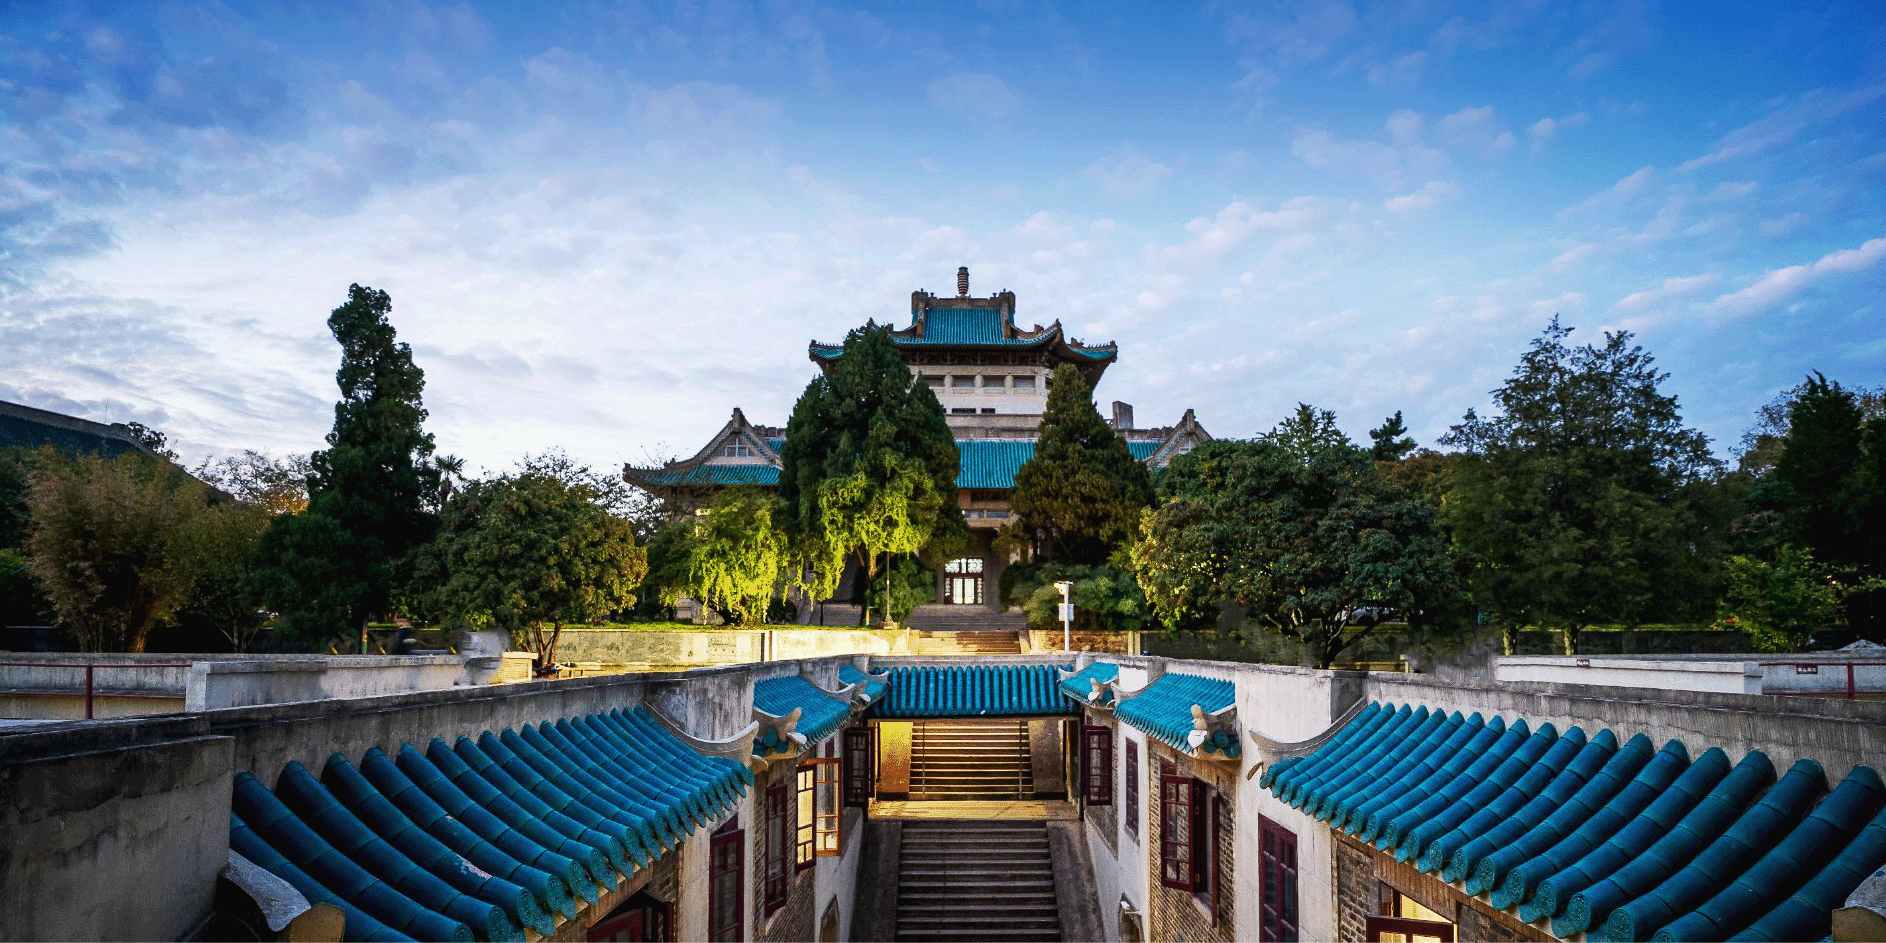
\includegraphics[width=0.6\paperwidth]{source/back1.png}
            \caption{樱顶的夜空}
        \end{figure}
        \begin{itemize}
            \item 没有标题的页面。
            \item 一份简短的入门,涵盖了公式、代码、分栏、表格、图片、参考文献\cite{key}。
            \item \textcolor{whugreen}{\large Good Luck}
        \end{itemize}
    \end{frame}
\endgroup
\section{References}
\begin{frame}{References}
\nocite{*}%让所有未被引用的文献都列出
%\addcontentsline{toc}{section}{References}
\printbibliography
\end{frame}
\end{document}
